% !TeX spellcheck = ru_RU
\documentclass{beamer}
\setbeamertemplate{navigation symbols}{}


\usetheme{Frankfurt}

\usepackage{amsmath,amssymb,amsthm,amscd,amsfonts}
\usepackage[utf8]{inputenc}
\usepackage[english, russian]{babel}
\usepackage{wrapfig}

\makeatletter
\newcommand*{\rom}[1]{\expandafter\@slowromancap\romannumeral #1@}
\makeatother


\newtheorem{definition_}{Определение}
\newtheorem{target_}{Цель работы}
\newtheorem{prob_}{Вероятностная постановка задачи классификации}
\newtheorem{algo_}{Алгоритмическая постановка задачи классификации}


\begin{document}
	\title{Синолитические сети в классификации мозговой активности}  
	\author{Власенко Даниил\\
	{\footnotesize Научные руководители: Гудкин Борис, Заикин Алесей}}
	\date{\today} 
	
	\begin{frame}
		\titlepage
	\end{frame}

	\begin{frame}
		\frametitle{Содержание}
		\tableofcontents
	\end{frame} 

	\section{Введение} 
	\begin{frame}
		\frametitle{фМРТ} 
							
		\begin{definition_}
			Функциональная магнитно-резонансная томография или фМРТ — разновидность магнитно-резонансной томографии (получения изображения), которая проводится с целью измерения нейронной активности головного или спинного мозга.
		\end{definition_}
	
		\begin{figure}
			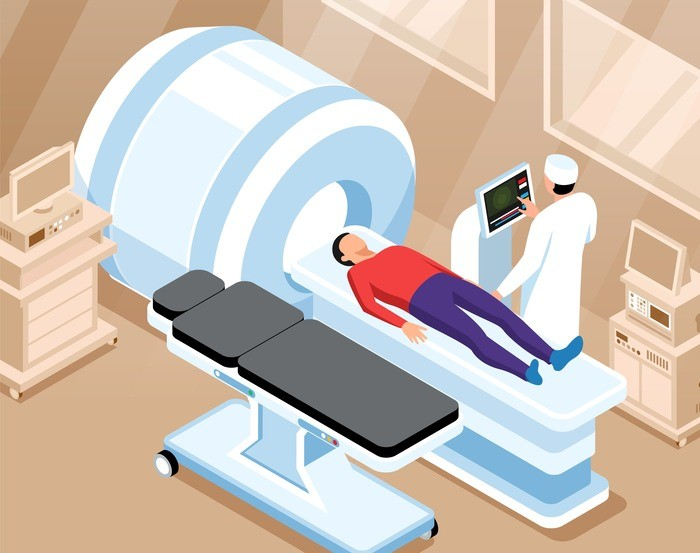
\includegraphics[width=4cm]{../images/fmri_1.jpeg}
			\caption{фМРТ сканер.} 
			\label{fg:1}
		\end{figure}		
	\end{frame}

	\begin{frame} 
		\frametitle{фМРТ}
		\begin{figure}
			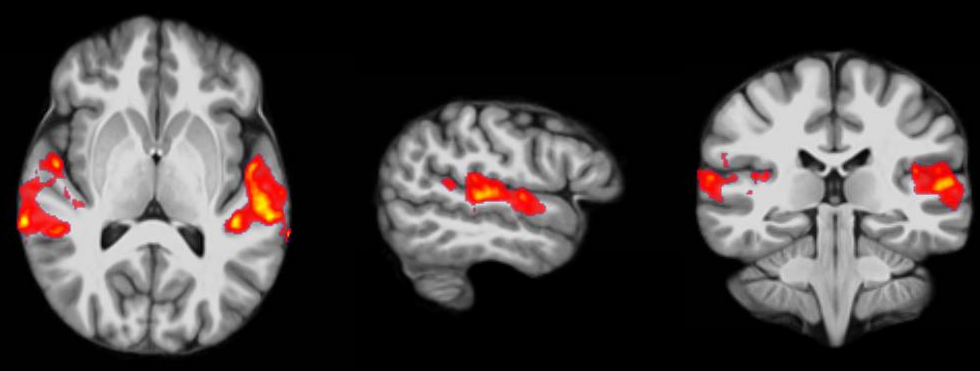
\includegraphics[width=10cm]{../images/fmri_2.png}
			\caption{фМРТ скан.} 
			\label{fg:2}
		\end{figure}
	\end{frame}

	\begin{frame} 
		\frametitle{Цель работы}
		Пусть мозг может находиться в двух режимах когнитивной деятельности. 
		
		\begin{target_}
			Реализация и тестирование нового метода классификации режимов когнитивной деятельности на основе фМРТ данных.
		\end{target_}			
	\end{frame}

	\section{Классификация}
	\begin{frame} 
		\frametitle{Задачи классификации}
		\begin{prob_}
			Пусть есть с.в. $\xi: \Omega \rightarrow X$ и с.в. $\eta: \Omega \rightarrow Y$. Рассмотрим с.в. $(\xi, \eta): \Omega \rightarrow (X, Y)$ с распределением $p(x, y)$.
			\vspace{0.5cm}
			
			Задача классификации сводится оценке $p(y|x)$ по выборке $D = \{(x_{k}, y_{k}), k = 1, \dots N\}$
		\end{prob_}
	
		\begin{algo_}
			Пусть $X$ --- множество описаний объектов, $Y$ --- множество номеров классов. Существует функция $f: X \rightarrow Y$, значения которой известны только на объектах конечной выборки $(X^{n}, Y^{n}) = \{(x_{1}, y_{1}), \dots, \{(x_{n}, y_{n})\}$. 
			\vspace{0.5cm}
			
			Требуется построить алгоритм-оценку $\widehat{f}: X \rightarrow Y$.
		\end{algo_}
	\end{frame}
	
	\section{Сенолитические сети}
	\begin{frame} 
		\frametitle{Основная идея}
		\begin{figure}
			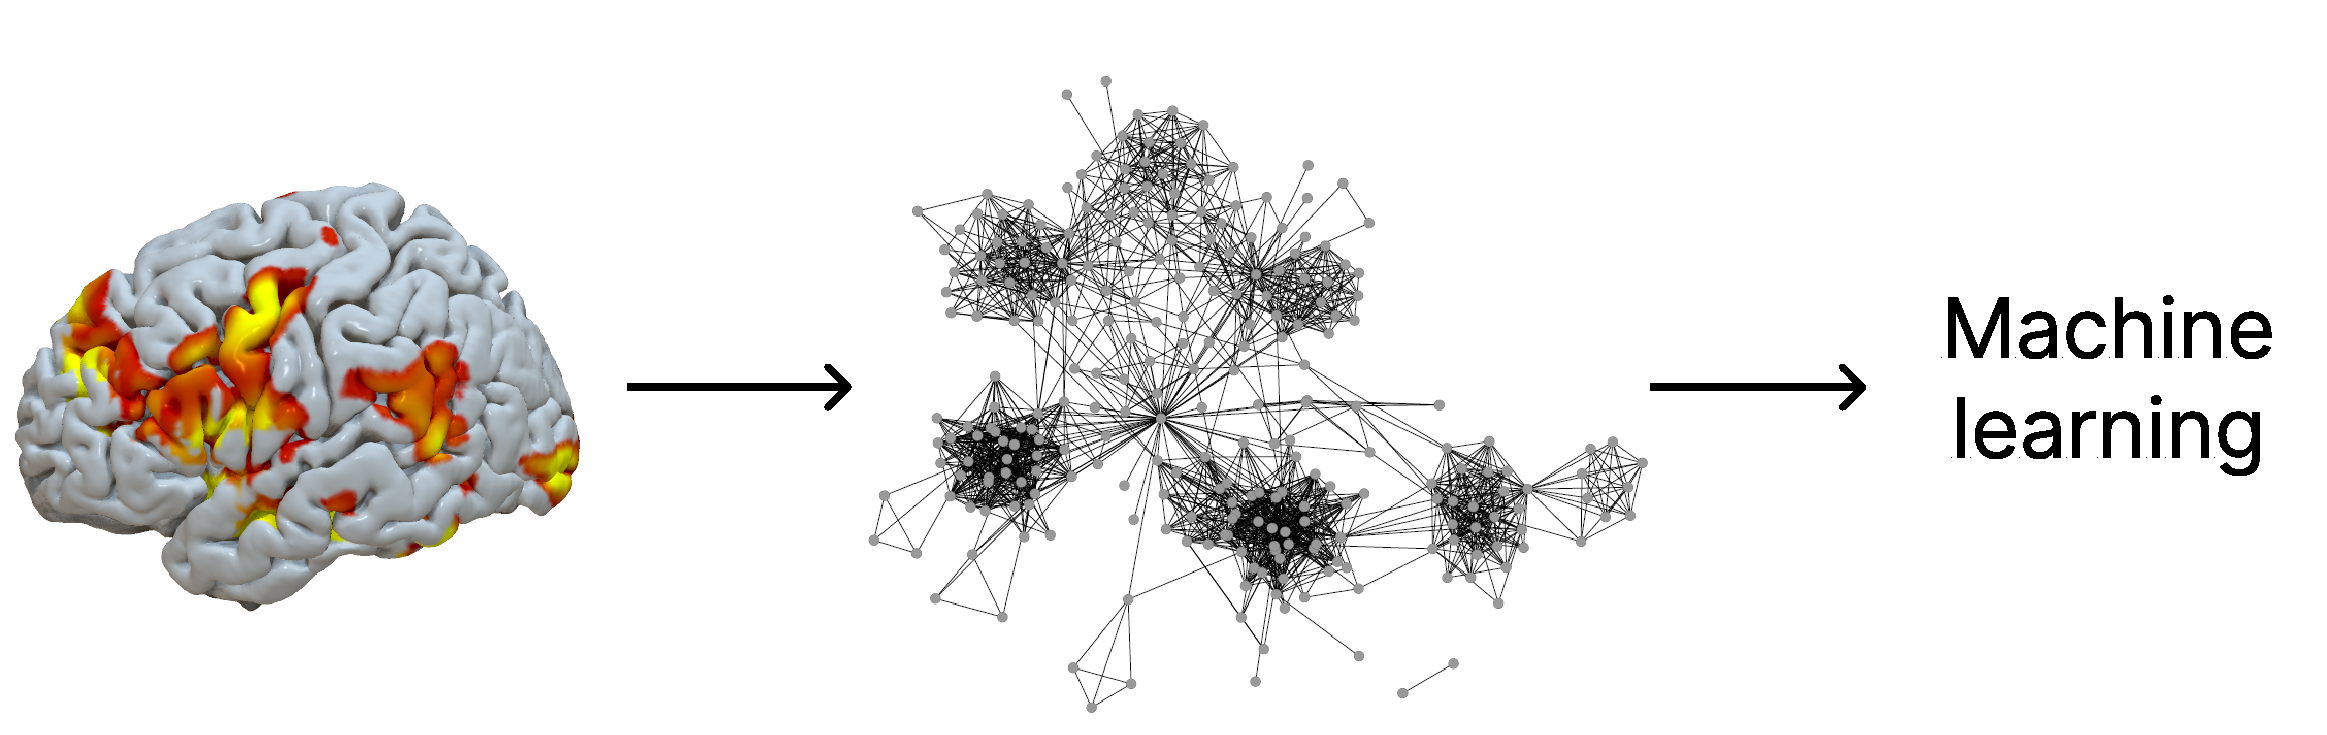
\includegraphics[width=10cm]{../images/fmri_graph_ml_1.pdf}
			\caption{Классификация на основе построения графов отражающих входные данные.} 
			\label{fg:3}
		\end{figure}
	\end{frame}

	\begin{frame} 
		\frametitle{Обозначения}
		Пусть $X = \{x_k\}_k$ --- множество фМРТ, а $Y = \{\rom{1}, \rom{2}\}$ --- множество режимов когнитивной активности.
		\vspace{0.5cm}
		
		На основе $x_k \in X$ строиться граф $G_k = (V_k, E_k, R_k W_k)$, где 
		\begin{itemize}
			\item $V_k = \{v_i^k\}_i$ --- множество вершин,
			\item $E_k = \{e_{ij}^k\}_{ij}$ --- множество неориентированных ребер,
			\item $R_k = \{r_i^k\}_i$ --- множество значений вершин,
			\item $W_k = \{w_{ij}^k\}_{ij}$ --- множество весов ребер,
			\item $v_i^k$ --- вершина отражающая область мозга $i$,
			\item $e_{ij}^k$ --- ребро отражающее связь между областями $i$ и $j$,
			\item $r_i^k$ -- значение вершины $v_i^k$,
			\item $w_{ij}^k$ -- вес ребра $e_{ij}^k$.
		\end{itemize}									
	\end{frame}

	\begin{frame} 
		\[
			w_{ij}^k = P(y_k = \rom{2} | r_i^k, r_j^k, (X^{n}, Y^{n})) - P(y_k = \rom{1} | r_i^k, r_j^k, (X^{n}, Y^{n}))
		\]
		\frametitle{Сенолитические сети}
		
		\begin{figure}
			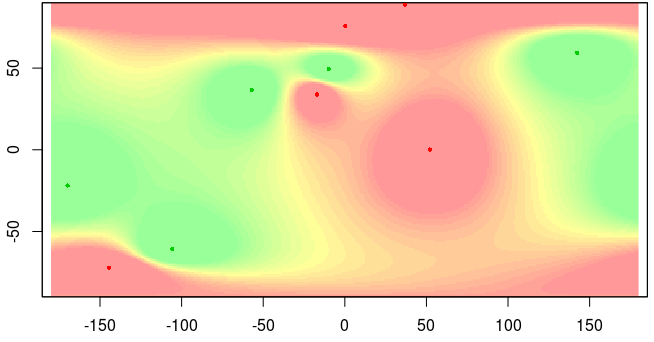
\includegraphics[width=10cm]{../images/classification.png}
			\caption{Вес ребер как вероятность режима.} 
			\label{fg:3}
		\end{figure}
	\end{frame}
		
		


\end{document}
	